\section{Lecture 16: Backpropagation and adjoints}
 From now onwards, we give up the luxuries afforded by convexity and move to the realm of non-convex functions. In the problems we have seen so far, deriving a closed-form expression for the gradients was fairly straightforward. But, doing so can be a challenging task for general non-convex functions. In this class, we are going to focus our attention on functions that can be expressed as compositions of multiple functions. In what follows, we will introduce \textit{backpropagation} - a popular technique that exploits the composite nature of the functions to compute gradients incrementally. 

\subsection{Warming up}
A common view of backpropagation is that ``\textit{it's just chain rule}''. 
This view is not particular helpful, however, and we will see that there is more
to it. As a warm-up example, let us look at the following optimization problem
with $g: \R^n \rightarrow \R$, $f: \R \rightarrow \R$:
\begin{align}
\min_{x} f(g(x)).
\end{align}
Using a similar trick to the one we saw in the context of ADMM, we can rewrite this problem as
\begin{align}
\min_{x} f(z) \\
\text{s.t.} \ \ z = g(x) \nonumber 
\end{align}
Note that we have converted our original unconstrained problem in $x$ into a constrained optimization problem in $x$ and $z$ with the following Lagrangian,
\begin{equation}
\mathcal{L} (x, z, \lambda) = f(z) + \lambda(g(x) - z).
\end{equation}
Setting $\nabla \mathcal{L} = 0$,  we have the following optimality conditions,
\begin{subequations}
\label{eq:opt}
\begin{align}
0 &= \nabla_x \mathcal{L} = \lambda g'(x) \Leftrightarrow 0 = \lambda g'(x) \label{eq:optx} \\
0 &= \nabla_z \mathcal{L} = f'(z) - \lambda \Leftrightarrow \lambda = f'(z) \label{eq:optz} \\
0 &= \nabla_{\lambda} \mathcal{L} = g(x) - z \Leftrightarrow z = g(x) \label{eq:optlambda}
\end{align}
\end{subequations}
which implies 
\begin{align}
0 &= f'(g(x))g'(x) \nonumber \\
&= \nabla_x f(g(x)) \nonumber \qquad \text{(by chain rule)} 
\end{align}
Hence, solving the Lagrangian equations gave us an incremental way of computing
gradients. As we will see shortly, this holds at great generality. It is
important to notice that we did \textit{not} use the chain rule when solving the
equations in~\eqref{eq:opt}. The chain rule only showed up in the proof of
correctness.

\subsection{General formulation}
Any composite function can be described in terms of its computation graph. As
long as the elementary functions of the computation graph are differentiable, we can perform the same procedure as above. Before moving ahead, let us introduce some notation: 
\begin{itemize}
\item Directed, acyclic computation graph: $\mathcal{G} = (\cV, \cE)$
\item Number of vertices: $|V| = n$
\item Set of ancestors of $i^{th}$ node: $\alpha(i) = \{ j \in \cV: (j, i) \in \cE\}$
\item Set of successors of $i^{th}$ node: $\beta(i) = \{ j\in \cV: (i, j) \in \cE\}$
\item Computation at the $i^{th}$ node: $f_i(z_{\alpha(i)})$, $\quad f_i: \R^{|\alpha(i)|} \rightarrow \R^{|\beta(i)|}$
\item Nodes:
\begin{itemize}
\item Input - $z_1,\dots,z_ d$
\item Intermediate - $z_{d+1}, \dots, z_{n-1}$
\item Output - $z_n$
\end{itemize}
\end{itemize}

\begin{figure}
 \centering
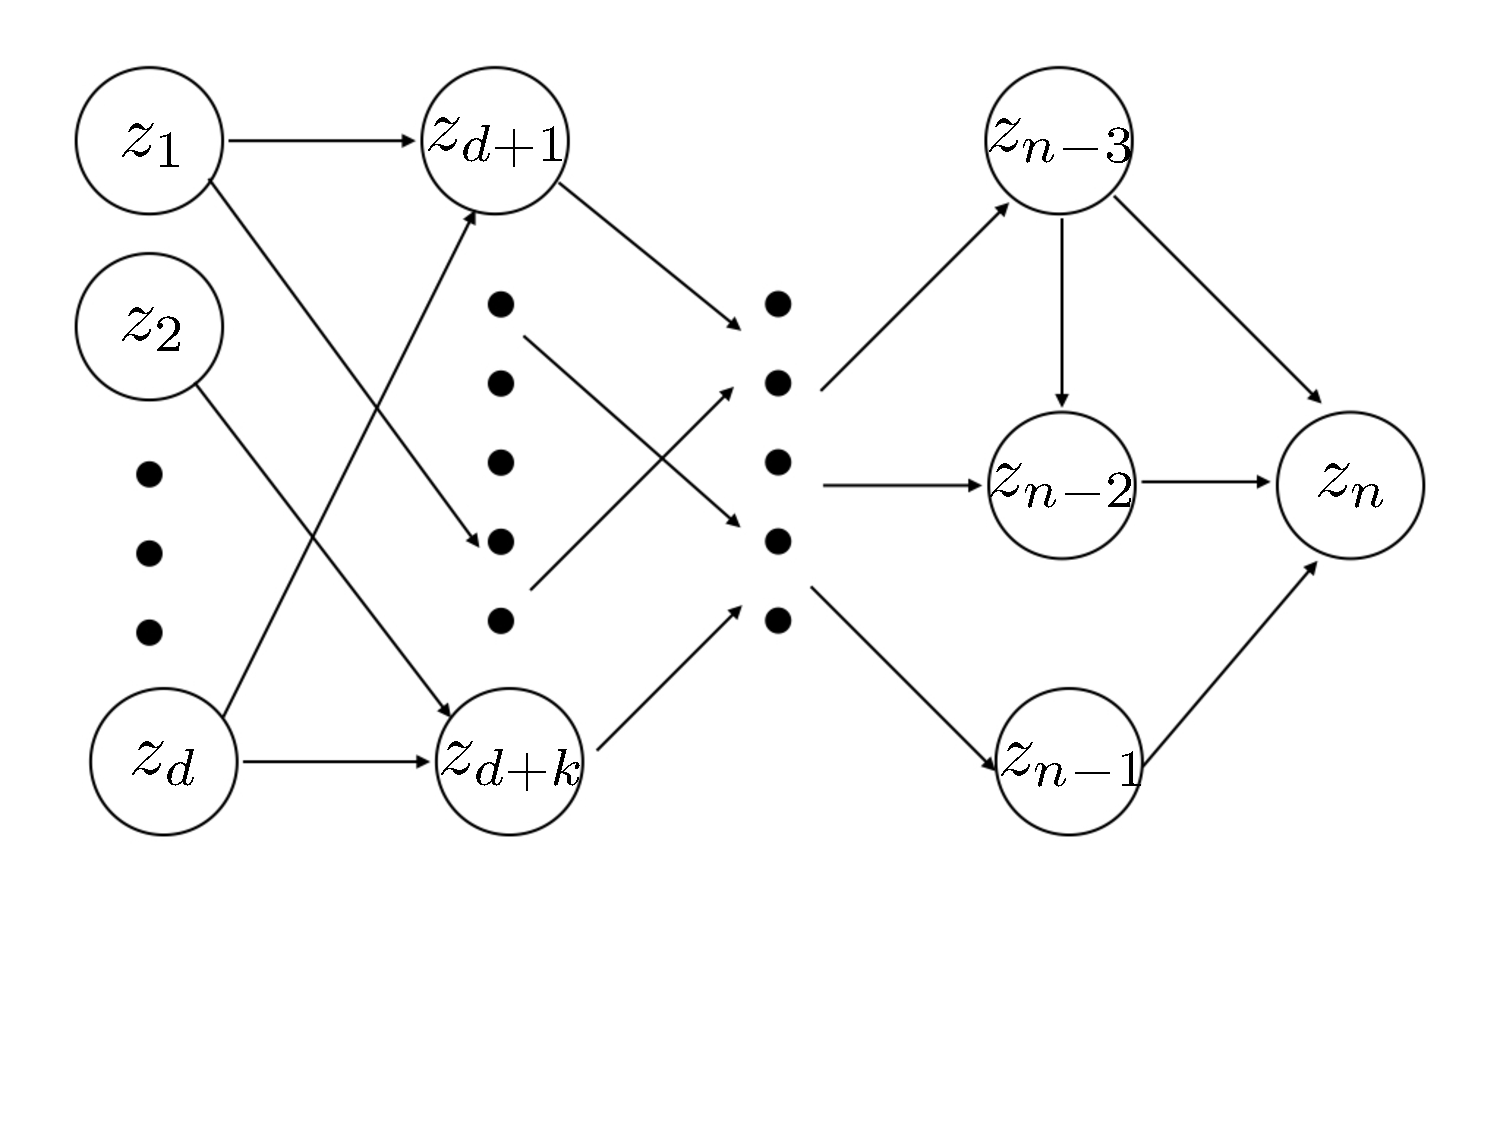
\includegraphics[width=0.7\linewidth, height=0.4\linewidth]{figures/lecture16_computation_graph.pdf} 
\label{fig:subim1}
\caption{Computation graph}
\end{figure}
\noindent
Then, the general formulation is given by
\begin{align}
&\min \ \ z_n \\
\text{s.t.} \ \ &z_i = f_i(z_{\alpha(i)}). \nonumber
\end{align}
with the following Lagrangian,
\begin{equation}
\mathcal{L}(x, z, \lambda) = z_n - \sum_{i} \lambda_i (z_i - f_i(z_{\alpha(i)})).
\end{equation}
As in the warmup example, we set $\nabla \mathcal{L} = 0$. This can be viewed as an algorithm comprising two separate steps:
\subsubsection*{Backpropagation algorithm}
\begin{itemize}
\item \textit{Step 1}: Set $\nabla_{\lambda} \mathcal{L} = 0$, i.e.,
\begin{align}
\nabla_{\lambda_i} \mathcal{L} = z_i - f_i(z_{\alpha(i)}) = 0 \Leftrightarrow z_i = f_i(z_{\alpha(i)})
\end{align}
\textit{Observation}: This is known as \textit{forward pass or forward propagation} as the values at the nodes ($z_i$) are computed using the values of the ancestors.
\item \textit{Step 2}: Set $\nabla_{z_j} \mathcal{L} = 0$, 
\begin{itemize}
\item for $j = n$, 
\begin{align*}
0 &= \nabla_{z_j} \mathcal{L} = 1 - \lambda_n \\
&\Leftrightarrow \lambda_n = 1
\end{align*}
\item for $j < n$,
\begin{align}
0  &= \nabla_{z_j} \mathcal{L} \nonumber \\
&=  \nabla_{z_j} (z_n - \sum_i \lambda_i (z_i - f_i(z_{\alpha(i)}))) \nonumber \\
&= - \sum_i \lambda_i (\nabla_{z_j} [z_i] - \nabla_{z_j} f_i(z_{\alpha(i)})) \nonumber \\
&= -\lambda_j + \sum_i \lambda_i \nabla_{z_j} f_i(z_{\alpha(i)}) \nonumber \\
&= -\lambda_j + \sum_{i \in \beta(j)} \lambda_i \frac{\partial f_i(z_{\alpha(i)})}{\partial z_j} \nonumber \\
\Leftrightarrow\quad \lambda_j &= \sum_{i \in \beta(j)} \lambda_i \frac{\partial f_i(z_{\alpha(i)})}{\partial z_j} \nonumber
\end{align}
\end{itemize}
\textit{Observation}: This is known as \textit{backward pass or backpropagation} as $\lambda_i's$ are computed using the gradients and values of $\lambda$ at successor nodes in the computation graph. 
\end{itemize}


\subsection{Connection to chain rule}
In this section, we will prove a theorem that explains why backpropagation allows us to calculate gradients incrementally.
\begin{theorem}
For all $1 \leq j \leq n$, we have
\begin{align*}
\lambda_j = \frac{\partial f(x)}{\partial z_j},
\end{align*}
i.e., the partial derivative of the function $f$ at x w.r.t to the $j^{th}$ node in the graph.
\end{theorem}

\begin{proof}
We assume for simplicity that the computation graph has $L$ layers and edges exist only between consecutive layers, i.e., $f = f_L \circ \dots \circ f_1 $. The proof is by induction over layers (starting from the output layer). \\
\medskip
\textit{Base case}: $\lambda_n = 1 = \frac{\partial f_n (x)}{\partial z_n} = \frac{\partial z_n}{z_n}$. \\
\medskip
\textit{Induction}: Fix $p^{th}$ layer and assume claim holds for nodes in all subsequent layers $l > p$.  Then, for node $z_j$ in layer $p$, 
\begin{align*}
\lambda_j &= \sum_{i \in \beta(j)} \lambda_i \frac{\partial f_i(z_{\alpha (i)})}{\partial z_j} \\
&= \sum_{i \in \beta(j)} \frac{\partial f(x)}{\partial z_i} \frac{\partial z_i}{z_j} \qquad (z_{\beta (j)} \text{ belong to layer } p+1) \\
&= \frac{\partial f(x)}{\partial z_j} \qquad \text{(by multivariate chain rule)}.
\end{align*}
\end{proof}
\noindent ($\ast$) Note that the proof for arbitrary computation graphs is by induction over the partial order induced by the reverse computation graph. 
\subsubsection*{Remarks}
\begin{enumerate}
\item Assuming elementary node operations cost constant time, cost of both the forward and backward pass is $O(|\mathcal{V}| + |\mathcal{E}|)$ $\Rightarrow$ Linear time!
\item Notice that the algorithm itself does not use the chain rule, only its correctness guarantee uses it. 
\item Algorithm is equivalent to the ``\textit{method of adjoints}'' from control theory introduced in the 60's. It was rediscovered by Baur and Strassen in '83 for computing partial derivatives \cite{baur1983complexity}. More recently, it has received a lot of attention due to its adoption by the Deep Learning community since the 90's.
\item This algorithm is also known as \textit{automatic differentiation}, not to be confused with 
\begin{enumerate}
\item Symbolic differentiation
\item Numerical differentiation
\end{enumerate}
\end{enumerate}

\subsection{Working out an example}
Suppose we have a batch of data $X \in \cR^{n \times d}$ with labels $y \in \cR^n$. Consider a two-layer neural net given by weights $W_1, W_2 \in \cR^{d \times d}: $
\begin{align*}
f(W_1,W_2) = \|\sigma(XW_1)W_2 -y\|^2
\end{align*}
To compute gradients, we only need to implement forward/backward pass for the elementary operations:
\begin{itemize}
\item Squared norm
\item Subtraction/addition
\item Component-wise non-linearity $\sigma$
\item Matrix multiplication
\end{itemize}
Observe that the partial derivatives for the first three operations are easy to compute. Hence, it suffices to focus on matrix multiplication. The two steps of the backpropagation algorithm in this context are:
\\
\textit{Forward Pass:}
\begin{itemize}
\item Input: $A \in \cR^{m \times n}, B \in \cR^{n \times d}$
\item Output: $C = AB \in \cR^{m \times d}$
\end{itemize}
\textit{Backward Pass:}
\begin{itemize}
\item Input: Partial derivatives $\Lambda \in \cR^{m \times d}$ (also $A,B,C$ from forward pass)
\item Output:
 \begin{itemize}
\item $\Lambda_1 \in \cR^{m \times n}$ (partial derivatives for left input)
\item $\Lambda_2 \in \cR^{n \times d}$ (partial  derivatives for right input)
\end{itemize}
\end{itemize}

\begin{claim}
$\Lambda_1 = \Lambda B^T, \Lambda_2 = A^T \Lambda$
\end{claim}

\begin{proof}
\begin{align*}
f &= \sum_{i,j} \lambda_{ij} C_{ij} = \sum_{i,j} (AB)_{ij} = \sum_{i,j} \lambda_{ij} \Sigma_k a_{ik}b_{kj}.
\end{align*}
So, by Lagrange update rule, 
\begin{align*}
(\Lambda_1)_{pq} &= \frac{\partial f}{\partial a_{pq}} = \sum_{i,j,k} \lambda_{ij} \frac{\partial a_{ik}}{\partial a_{pq}} b_{kj} = \sum_j \lambda_{pj} b_{qj} = (\Lambda B^T)_{pq}.
\end{align*}
Using the same approach for partial derivative w.r.t. $B$, we get 
\begin{align*}
(\Lambda_2)_{pq} = (A^T \Lambda)_{pq}
\end{align*}
\end{proof}
